\documentclass{uimppracticas}

%Permitir cabeceras y pie de páginas personalizados
\pagestyle{fancy}

%Path por defecto de las imágenes
\graphicspath{ {./images/} }

%Declarar formato de encabezado y pie de página de las páginas del documento
\fancypagestyle{doc}{
  %Pie de Página
  \footerpr{}{}{{\thepage} de \pageref{LastPage}}
}

%Declarar formato de encabezado y pie del título e indice
\fancypagestyle{titu}{%
  %Cabecera
  \headerpr{}{}{}
  %Pie de Página
  \footerpr{}{}{}
}

\appto\frontmatter{\pagestyle{titu}}
\appto\mainmatter{\pagestyle{doc}}

\begin{document}
	
%Comienzo formato título
\frontmatter

%Portada (Centrado todo)
\centeredtitle{./images/LogoUIMP.png}{Máster Universitario en Investigación en Inteligencia Artificial}{Curso 2020-2021}{Recuperación y extracción de información, \\ grafos y redes sociales}{Análisis y Visualización Básica de una Red Social con Gephi}

\begin{center}
\large \today
\end{center}

\vspace{40mm}

\begin{flushright}
 	{\bf Laura Rodríguez Navas}\\
 	\textbf{DNI:} 43630508Z\\
 	\textbf{e-mail:} \href{rodrigueznavas@posgrado.uimp.es}{rodrigueznavas@posgrado.uimp.es}
\end{flushright}

\newpage

%Índice
% \tableofcontents

% \newpage

%Comienzo formato documento general
\mainmatter

\setlength\parskip{2.5ex}

\section*{La Red}

La red \textit{Diseasome}\cite{Goh8685} seleccionada para realizar esta práctica es una red no dirigida de trastornos y genes de diferentes enfermedades vinculadas por asociaciones conocidas entre trastornos y genes, que nos indican el origen genético común de muchas enfermedades. La forman 526 enfermedades y 903 genes, donde los genes asociados con trastornos similares muestran una mayor probabilidad de interacciones físicas entre sus productos y una mayor similitud de perfiles de expresión para sus transcripciones, lo que respalda la existencia de distintos módulos funcionales específicos de la enfermedad. 

El conjunto de datos de \textit{Diseasome} viene como un archivo \textit{.zip}, que se puede descargar en el siguiente enlace: \url{http://gephi.org/datasets/diseasome.gexf.zip}. Una vez descargado y descomprimido, obtenemos un archivo \textit{.gexf}, que contiene un archivo de grafos. Importamos el archivo de grafos a \textit{Gephi}\cite{Gephi} y comenzamos a probar diferentes opciones de visualización.

Después de probar diferentes visualizaciones encojemos el algoritmo de distribución: Fruchterman Reingold (en la ventada \textit{Distribución}). Para evitar que las componentes conexas queden fuera de la vista principal, fijamos el valor del parámetro \textit{Gravedad} a 20. También marcamos las opciones \textit{Disuadir Hubs y/o Evitar el solapamiento}. Esto convierte la visualización en un círculo y coloca la red alrededor de la misma área (ver Figura \ref{completa_negro_FR}). 

De aquí pasamos a la detección de comunidades para colorear los clústers de la red. \textit{Gephi} implementa el método \href{https://es.wikipedia.org/wiki/M\%C3\%A9todo_de_Louvain}{Louvain} disponible en el panel de \textit{Estadísticas}. Damos clic en ejecutar \textit{Modularidad} y veremos como el algoritmo de detección de comunidades nos ha creado un nuevo parámetro de particionamiento (\textit{Modularity Class}). Si seleccionamos este nuevo parámetro observaremos las comunidades encontradas y si finalmente pulsamos \textit{Aplicar} colorearemos los nodos según las comunidades encontradas. Esto hace que la visualización sea más colorida y se vean bien donde se encuentra cada comunidad.

\begin{figure}[h]
	\centering
	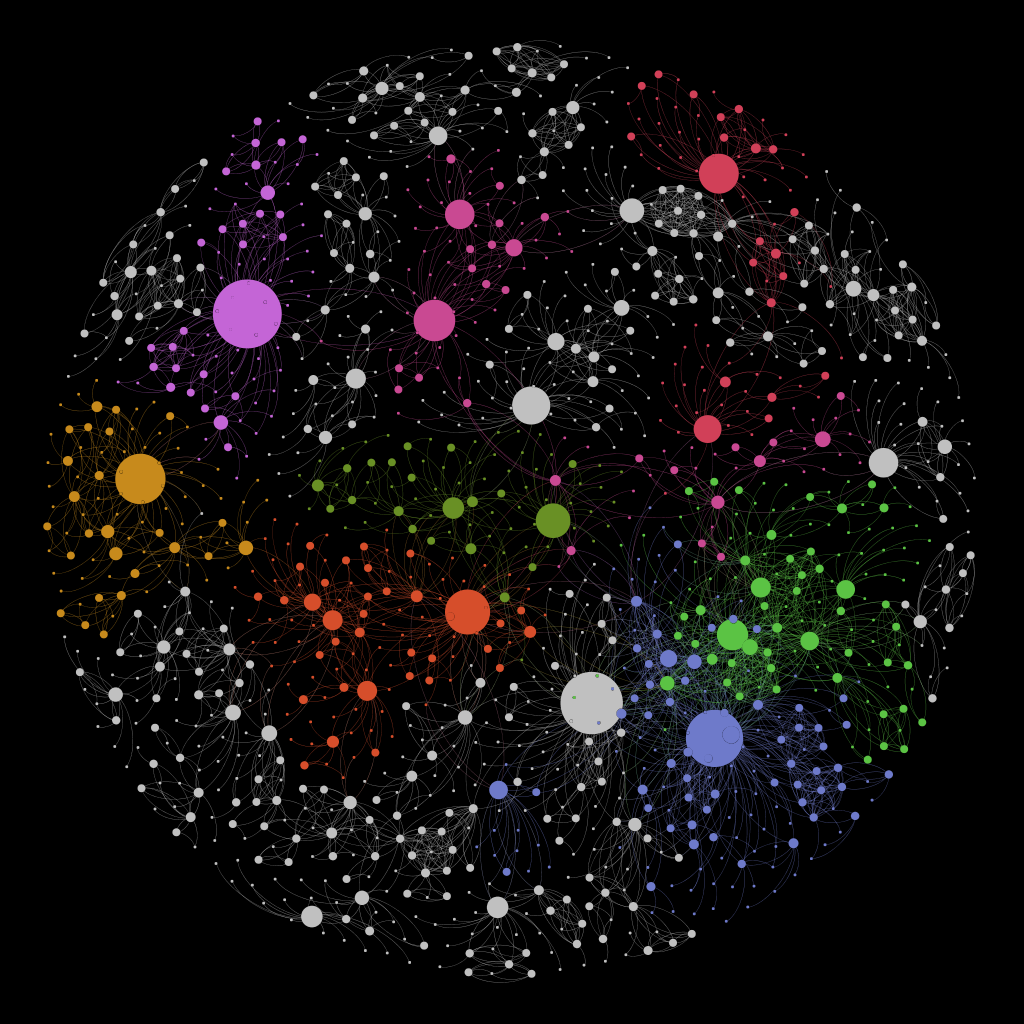
\includegraphics[width=0.6\textwidth]{images/completa_negro_FR}
	\caption{Red completa sobre un fondo negro sin etiquetas.}
	\label{completa_negro_FR}
\end{figure}

A continuación, añadiremos las etiquetas a los nodos para ver la red con más a detalle (ver Figura \ref{completa_FR_labels}). 

\begin{figure}[h]
	\centering
	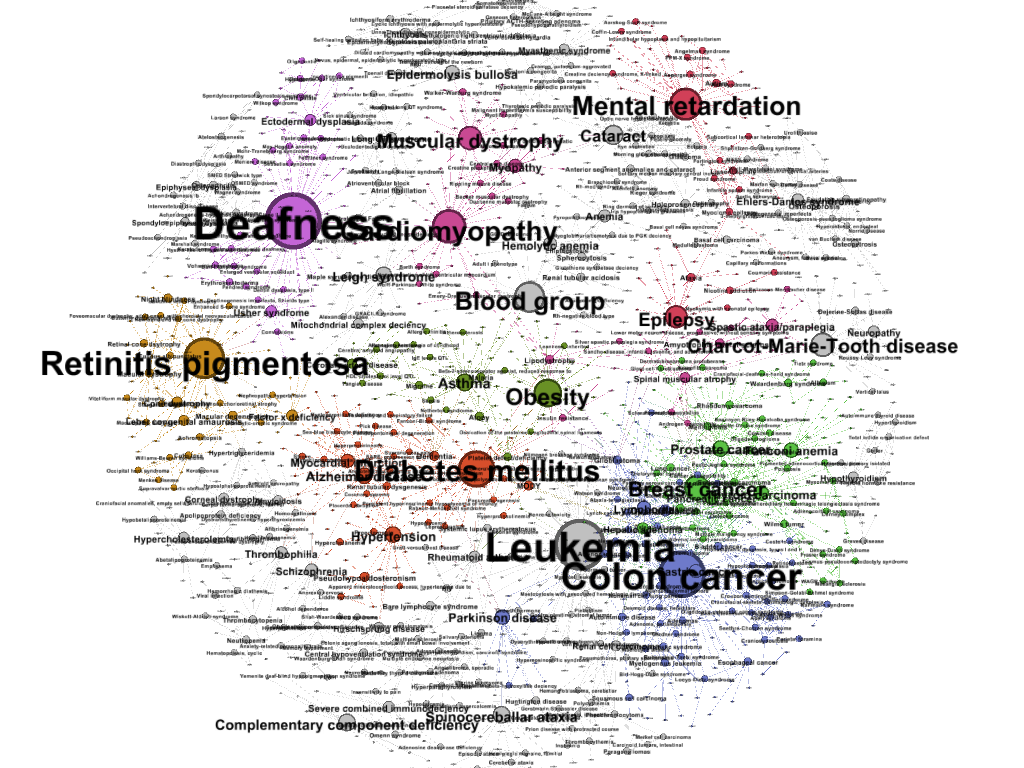
\includegraphics[width=0.9\textwidth]{images/completa_FR_labels}
	\caption{Red completa sobre un fondo blanco con etiquetas.}
	\label{completa_FR_labels}
\end{figure}

Las diferentes comunidades están agrupadas por colores. El tamaño de las etiquetas depende del tamaño del nodo. Está claro que los cánceres son la enfermedad más dominante de todas, es una de las enfermedades más comunes en comparación con otras que existen en la actualidad. La sordera es la enfermedad que se lleva la mayor porción. También vemos diferentes clústers además de los cánceres, como la diabetes, la salud mental, etc. 

\section*{Análisis Básico de la Red}

Para los primeros pasos del análisis de la red, comenzamos por anotar los valores de las medidas globales básicas: el número de nodos 1419 ($N$) y el número de enlaces 3926 ($L$), que aparecen directamente en la ventana Contexto, además de calculamos manualmente el número máximo de enlaces $L_{max}$. 

Posteriormente, calculamos otra medida global, el grado medio <k>, ejecutando la opción correspondiente en la ventana \textit{Estadísticas}. El valor del grado medio <k> es 5,533. Al realizar el cálculo del grado medio, también obtenemos la distribución de grados de la red completa (ver Figura \ref{degree-distribution}).

\begin{figure}[h]
	\centering
	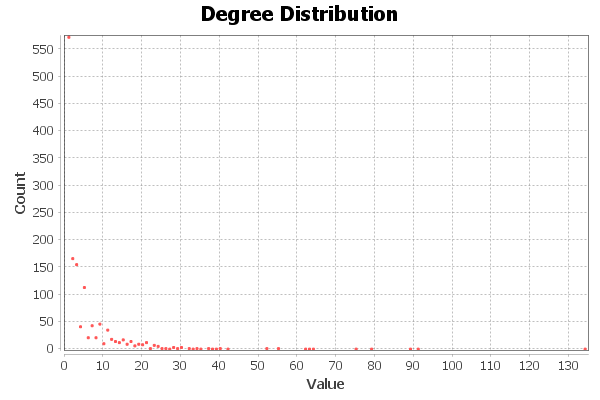
\includegraphics[width=0.6\textwidth]{images/degree-distribution}
	\caption{Distribución de grados de la red completa.}
	\label{degree-distribution}
\end{figure}

\begin{center}
	$L_{max} = N * (N-1) = 1419 * (1419 - 1) = 2012142$
\end{center}

\section*{Estudio de la Centralidad de los Actores}

\section*{Visualizaciones y Gráficos adicionales}

%\section*{Conclusiones}
%
%Gephi definitivamente tiene una curva de aprendizaje. Aunque hay tutoriales que son fáciles de seguir, a veces la visualización no sale como yo quería. Tampoco es el software más intuitivo porque no tiene una función de deshacer. El archivo Gephi debe guardarse constantemente cada vez que se renderiza una nueva visualización. Incluso con tanta frustración con el software, me encantó probar nuevas visualizaciones para ver cómo resultaban.
%
%Si tuviera que ampliar este proyecto, intentaría buscar otros diseños, por ejemplo, un diseño circular y crear una red desde allí. También me gustaría aprender a hacer el limpiador visual. Hice todo lo posible para dejarlo claro en mi visualización actual, pero me gustaría mejorarlo más. Creo que hay potencial. Agregar interacción al mapa también sería una opción.

\newpage

\renewcommand{\refname}{Bibliografía}
\bibliographystyle{unsrt}
\bibliography{biblio}

\end{document}
